\documentclass[12pt]{article}

\usepackage{graphicx}
\usepackage{booktabs}
\usepackage{float}
\usepackage{geometry}
\usepackage{hyperref}

\geometry{margin=1in}

\title{Evaluation of Classical Edge Detection Methods}
\author{Amirreza Rajabi}
\date{\today}

\begin{document}

\maketitle

\section{Introduction}

Edge detection is a fundamental task in image processing and computer vision. 
It aims to identify significant intensity changes in an image, which often correspond to object boundaries. 
In this project, several classical edge detection methods are evaluated, including Sobel, Roberts, Prewitt, Canny, and Laplacian of Gaussian (LoG).
The evaluation is performed using both quantitative metrics and qualitative visual comparison.

\section{Edge Detection Methods}

\begin{itemize}
\item \textbf{Sobel}: Uses first-order derivatives to detect horizontal and vertical edges.
\item \textbf{Roberts}: A simple gradient-based operator using diagonal differences.
\item \textbf{Prewitt}: Similar to Sobel but with uniform weights, emphasizing edge direction.
\item \textbf{Canny}: A multi-stage detector designed for optimal edge detection with noise suppression.
\item \textbf{LoG}: Combines Gaussian smoothing with second-order derivatives for edge detection.
\end{itemize}

\section{Evaluation Metrics}

The performance of each method is evaluated using the following metrics:

\begin{itemize}
\item \textbf{Precision}: Measures the proportion of detected edges that are correct.
\item \textbf{Recall}: Measures the proportion of ground-truth edges that are detected.
\item \textbf{F1-score}: The harmonic mean of precision and recall.
\item \textbf{Accuracy}: The overall correctness of edge detection results.
\end{itemize}

\section{Quantitative Results}

Table~\ref{tab:quant_results} shows the quantitative comparison of the evaluated edge detection methods.

\begin{table}[H]
\centering
\caption{Quantitative comparison of edge detection methods}
\label{tab:quant_results}
\begin{tabular}{lcccc}
\toprule
\textbf{Method} & \textbf{Precision} & \textbf{Recall} & \textbf{F1-score} & \textbf{Accuracy} \\
\midrule
Sobel   & 0.1042 & 0.3762 & 0.1534 & 0.0852 \\
Roberts & 0.0740 & 0.1957 & 0.0984 & 0.0526 \\
Prewitt & 0.1051 & 0.3847 & 0.1554 & 0.0864 \\
Canny   & 0.1528 & 0.1098 & 0.1169 & 0.0628 \\
LoG     & 0.0649 & 0.5287 & 0.1111 & 0.0600 \\
\bottomrule
\end{tabular}
\end{table}

\section{Qualitative Results}

\subsection{Results on Proposed Dataset}

Figure~\ref{fig:own_edge_comparison} shows a visual comparison of edge detection methods on sample images from the proposed dataset. 
Sobel and Prewitt produce relatively continuous and strong edges, while Canny generates thin and clean edges but misses some weak boundaries. 
LoG detects a large number of edges, including noise, whereas Roberts produces sparse and fragmented results.

\begin{figure*}[t]
\centering
\begin{tabular}{cccccc}
\textbf{Image} & \textbf{Sobel} & \textbf{Roberts} & \textbf{Prewitt} & \textbf{Canny} & \textbf{LoG}
\end{tabular}

\vspace{0.2cm}

\begin{tabular}{cccccc}
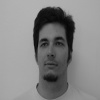
\includegraphics[width=0.14\textwidth]{../images/face.jpg} &

\includegraphics[width=0.14\textwidth]{../results/sobel/face.jpg} &

\includegraphics[width=0.14\textwidth]{../results/roberts/face.jpg} &

\includegraphics[width=0.14\textwidth]{../results/prewitt/face.jpg} &

\includegraphics[width=0.14\textwidth]{../results/canny/face.jpg} &

\includegraphics[width=0.14\textwidth]{../results/log/face.jpg}
\end{tabular}

\vspace{0.15cm}

\begin{tabular}{cccccc}
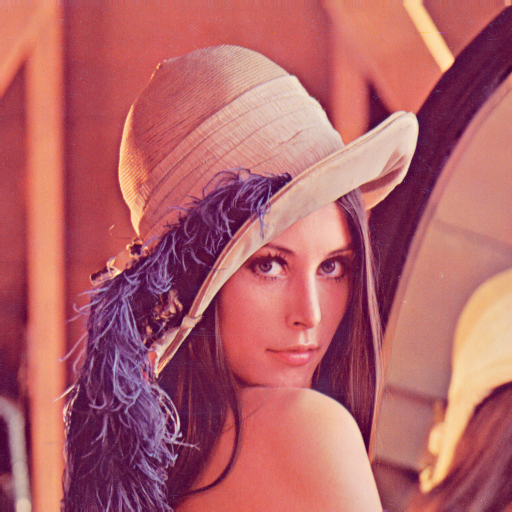
\includegraphics[width=0.14\textwidth]{../images/lena.png} &

\includegraphics[width=0.14\textwidth]{../results/sobel/lena.png} &

\includegraphics[width=0.14\textwidth]{../results/roberts/lena.png} &

\includegraphics[width=0.14\textwidth]{../results/prewitt/lena.png} &

\includegraphics[width=0.14\textwidth]{../results/canny/lena.png} &

\includegraphics[width=0.14\textwidth]{../results/log/lena.png}
\end{tabular}

\caption{Comparison of edge detection methods on samples from the proposed dataset.}
\label{fig:own_edge_comparison}
\end{figure*}

\subsection{Results on BSDS Dataset}

\textbf{Berkeley Segmentation Dataset and Benchmark (BSDS)} is a widely used dataset for evaluating edge detection and image segmentation algorithms. 
It consists of natural images along with multiple human-annotated ground-truth edge maps, capturing perceptually meaningful boundaries. 
The availability of multiple annotations makes BSDS a reliable benchmark for assessing the consistency and robustness of edge detection methods.

Figure~\ref{fig:bsds_edge_comparison} presents qualitative results on the BSDS dataset. 
The trends observed are consistent with the proposed dataset, confirming the general behavior of each method across different image distributions.

\begin{figure*}[t]
\centering
\begin{tabular}{ccccccc}
\textbf{Image} & \textbf{Sobel} & \textbf{Roberts} & \textbf{Prewitt} & \textbf{Canny} & \textbf{LoG} & \textbf{GT}
\end{tabular}

\vspace{0.2cm}

\begin{tabular}{ccccccc}
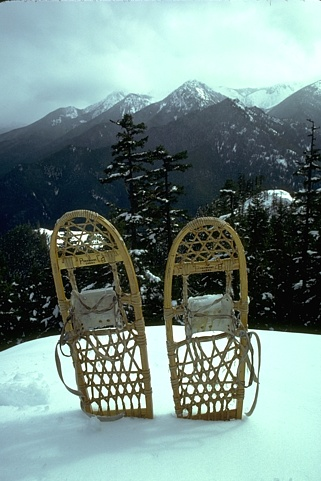
\includegraphics[width=0.14\textwidth]{../images/bsd1.jpg} &

\includegraphics[width=0.14\textwidth]{../results/sobel/bsd1.jpg} &

\includegraphics[width=0.14\textwidth]{../results/roberts/bsd1.jpg} &

\includegraphics[width=0.14\textwidth]{../results/prewitt/bsd1.jpg} &

\includegraphics[width=0.14\textwidth]{../results/canny/bsd1.jpg} &

\includegraphics[width=0.14\textwidth]{../results/log/bsd1.jpg} &
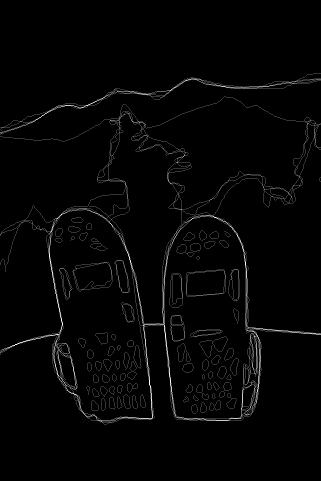
\includegraphics[width=0.14\textwidth]{../images/bsd1_gt.jpg}
\end{tabular}

\vspace{0.15cm}

\begin{tabular}{ccccccc}
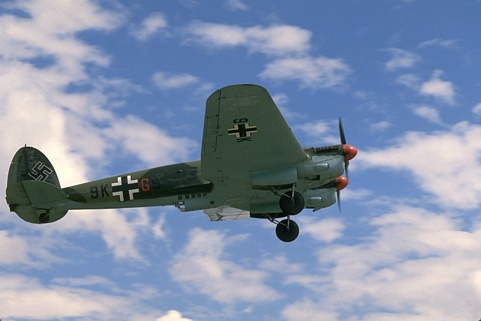
\includegraphics[width=0.14\textwidth]{../images/bsd2.jpg} &

\includegraphics[width=0.14\textwidth]{../results/sobel/bsd2.jpg} &

\includegraphics[width=0.14\textwidth]{../results/roberts/bsd2.jpg} &

\includegraphics[width=0.14\textwidth]{../results/prewitt/bsd2.jpg} &

\includegraphics[width=0.14\textwidth]{../results/canny/bsd2.jpg} &

\includegraphics[width=0.14\textwidth]{../results/log/bsd2.jpg} &
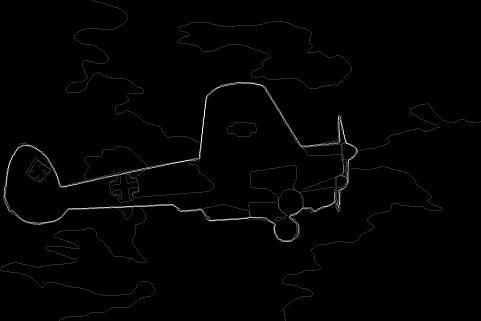
\includegraphics[width=0.14\textwidth]{../images/bsd2_gt.jpg}
\end{tabular}

\caption{Comparison of edge detection methods on samples from the BSDS dataset.}
\label{fig:bsds_edge_comparison}
\end{figure*}

\section{Conclusion}

This project presented a comparative evaluation of classical edge detection techniques using both quantitative metrics and qualitative visualization. 
Prewitt and Sobel achieved the best balance between precision and recall, while Canny provided clean but incomplete edges. 
LoG detected the most edges but introduced significant noise, and Roberts showed limited performance. 
These results highlight the trade-offs involved in selecting an edge detection method for practical applications.

\section{Future Work}

While classical edge detection methods provide valuable insights, their performance is inherently limited by hand-crafted filters and fixed parameters. 
Future work may focus on employing deep learning-based edge detection approaches, such as convolutional neural networks (CNNs), which can learn rich hierarchical features directly from data. 
Such methods have demonstrated superior robustness to noise, texture variations, and complex scene structures, and may significantly improve edge detection accuracy on challenging datasets.

\end{document}
